\documentclass[11pt]{article}
\usepackage[dvips]{graphicx, color}
\usepackage{epsfig}
\usepackage{amsmath}
\usepackage{mathptmx}

\setlength{\evensidemargin}{-0.7cm}
\setlength{\oddsidemargin}{-0.0cm}
\setlength{\textwidth}{15.5cm}
\setlength{\topmargin}{-2cm}
\setlength{\textheight}{23.5cm}
\parskip 1ex    % White space between paragraphs amount
\parindent 0pt

\usepackage{html}
\usepackage[ruled]{algorithm2e}
%\usepackage{varioref}
%\usepackage[breaklinks=true,pagebackref=true]{hyperref}
%\hypersetup{colorlinks=true,urlcolor=black,citecolor=blue}

\newcommand{\red}{\color{red}}
\newcommand{\green}{\color{green}}
\newcommand{\blue}{\color{blue}}

\graphicspath{{Figures/}}

\begin{document}

\title{MSTransform Framework in CASA}
\author{Sandra Castro and Justo Gonzalez}
\date{07 February 2013, (last modified : 16 December 2014)}
\maketitle

This memo describes the MSTransform module in CASA as available from version
4.1.0 onwards.
%Section \ref{Sec:CodeDocs} gives an outline of the software implementation. 
Section \ref{Sec:Running} 
describes what 
various transformations do, with some examples and suggestions on how to use them in
Section \ref{Sec:Examples}. 
Section \ref{Sec:FAQ} contains a list of frequently-asked questions and their answers.

This is a living document. Details will continue to be added (with examples). Feedback is welcome.

\tableofcontents

%\section{Software Documentation}

\subsection{C++ Infrastructure}\label{Sec:CodeDocs}

\subsubsection{Framework}
%{\green Link to (or copy of) Justo's documentation of the infrastructure design, 
%with links from each 'class' box/section to the relevant doxygen code-doc pages. }

\paragraph{Main Classes}

\begin{enumerate}
\item
%\htmladdnormallink{AgentFlagger}{http://www.eso.org/~scastro/ALMA/casa/active/CasaRef/agentflagger-Tool.html}:
%\htmladdnormallink{AgentFlagger}{http://casa.nrao.edu/active/docs/CasaRef/agentflagger-Module.html}:
\htmladdnormallink{AgentFlagger}{http://casa.nrao.edu/docs/CasaRef/agentflagger-Module.html}:
The top-level AgentFlagger class that connects all of the following together, and defines the C++ user-interface 
for the agentflagger.  
This is the class used by the tool layer.

%\item \htmladdnormallink{FlagDataHandler}{http://www.eso.org/~jagonzal/Flagging-3.4-Docs/html/classcasa_1_1FlagDataHandler.html} : A top level class defining the data handling interface for the flagging module. 
\item \htmladdnormallink{FlagDataHandler}{http://casa.nrao.edu/docs/doxygen/html/classcasa_1_1FlagDataHandler.html} : 
A top level class defining the data handling interface for the flagging module. 

\item The  \htmladdnormallink{FlagAgentBase}{http://casa.nrao.edu/docs/doxygen/html/classcasa_1_1FlagAgentBase.html} 
base class defines the behaviour of all flagging agents
and contains agent-level data-selection, etc.  The main functions to be implemented by derived classes are
setAgentParameters(), preProcessBuffer(), computeAntennaPairFlags() or computeRowFlags(), getReport() . 

List of available Flag Agents : 
\begin{enumerate}
\item \htmladdnormallink{FlagAgentManual}{http://casa.nrao.edu/docs/doxygen/html/classcasa_1_1FlagAgentManual.html} :  
Flag/Unflag based on data-selections.  
The only processing done by this agent is to set the flags for all data it sees to 
True if the operation is to flag, and to False to unflag. A boolean parameter
apply determines whether to flag (apply=True) or unflag (apply=False). By
default it is set to True.

\item \htmladdnormallink{FlagAgentQuack}{http://casa.nrao.edu/docs/doxygen/html/classcasa_1_1FlagAgentQuack.html} :  
Flag time-ranges at the beginning and/or end of scans. 
Uses the YYY iteration-mode. 

\item \htmladdnormallink{FlagAgentElevation}{http://casa.nrao.edu/docs/doxygen/html/classcasa_1_1FlagAgentElevation.html} : 
Flag time-ranges based on source elevation. 
Uses the YYY iteration-mode.

\item \htmladdnormallink{FlagAgentShadow}{http://casa.nrao.edu/docs/doxygen/html/classcasa_1_1FlagAgentShadow.html} : 
For each timestep, flag antennas that are shadowed by
any other antenna.  Antennas to be flagged are chosen and marked in the preProcess() stage.
Rows are flagged in computeRow(), and this agent uses the YYY iteration-mode.

\item \htmladdnormallink{FlagAgentExtend}{http://casa.nrao.edu/docs/doxygen/html/classcasa_1_1FlagAgentExtension.html} : 
Read and extend flags along specified axes, within the
current chunk.  Uses the YYY iteration-mode.

\item \htmladdnormallink{FlagAgentClip}{http://casa.nrao.edu/docs/doxygen/htmlclasscasa_1_1FlagAgentClipping.html} : 
Flag based on a clip threshold and visExpression.
Find and flag NaNs and Infs.  Uses the YYY iteration-mode. 

\item \htmladdnormallink{FlagAgentTimeFreqCrop}{http://casa.nrao.edu/docs/doxygen/html/classcasa_1_1FlagAgentTimeFreqCrop.html} : 
The TFCrop algorithm is run per
baseline, via FlagAgentTimeFreqCrop::computeAntennaPairFlags()

\item \htmladdnormallink{FlagAgentRFlag}{http://casa.nrao.edu/docs/doxygen/html/classcasa_1_1FlagAgentRFlag.html} : 
The RFlag algorithm. 
Implements multiple passes through each chunk via the  passIntermediate() and passFinal() mechanism.

\item \htmladdnormallink{FlagAgentSummary}{http://casa.nrao.edu/docs/doxygen/html/classcasa_1_1FlagAgentSummary.html} : 
Flag counts are accumulated in computeRow()
and packaged into a Record in getResult(). 

\item \htmladdnormallink{FlagAgentDisplay}{http://casa.nrao.edu/docs/doxygen/html/classcasa_1_1FlagAgentDisplay.html} : 
Visibilities are read and displayed from computeAntennaPair(). Navigation-buttons control the order in which the framework iterates through baselines. 

\end{enumerate}



\item The \htmladdnormallink{FlagReport}{http://casa.nrao.edu/docs/doxygen/html/classcasa_1_1FlagReport.html} class allows each flag agent to build and return 
information (summary counts, reports as plots, etc) to the user (and/or) to the display agent
for end-of-MS reports.
\end{enumerate}


\subsubsection{Control Flow}
%{\green  Justo, if you have a nicer way to describe the control flow, then please replace this part,  but otherwise, just this text-algorithm may be good-enough for this document (after it's completed).  If you already have the different iteration-modes explained somewhere (in one of the .h files), we can just point to it from here.  }


%%% For documentation on how to use this syntax, see the PDF file from here : 
%%  http://www.ctan.org/tex-archive/macros/latex/contrib/algorithm2e/

\begin{algorithm}
  \SetLine
%  \linesnumbered
  \dontprintsemicolon
  \vspace{0.5cm} 
  \KwData{Pre-selected Measurement Set}
  \KwIn{List of Flag Commands}
  \KwOut{Flags updated in-place + summaries/reports}
  \vspace{0.5cm} 
  {Setup FlagDataHandler :} \;
  {Build Agent List }\;
  \While (\tcc*[f]{chunks (array,obs,field,spw)}) { more chunks }
  {
    \While (\tcc*[f]{sub-chunks (ntime)}) { more times }
    {
      \ForAll (\tcc*[f]{agents}) { agents }
      {
        \If {agent touches this data}
        {
          {agent :: pre-Process current buffer}\;
             \If {iterationApproach = XXX}
             {
               \ForAll {baselines}
               {
                  {agent :: computeAntennaPairFlags()}\;
               }
             }
             \If {iterationApproach = YYY}
             {
               \ForAll {rows}
               {
                {agent :: computeRowFlags() }\;
               }
             }
        }
      }
    }
    {fdh :: Flush Flag Cube}\;
  }
  {Gather Reports from all agents} \;
\end{algorithm}





\subsubsection{Performance Optimizations}

%{\green  Explanation of various performance-optimization features  }


There are several performance-optimization choices that can be made. 
Some of these are under the users control, and some have automated heuristics.

\paragraph{List mode}

It helps to combine multiple flag commands into a single run ONLY if most of the
commands require the same data to be read.  

The goal is to read data once, apply multiple flag commands, and write flags once.

\begin{enumerate}
\item  Manual-flag commands read only meta-data.
\item  Shadow, elevation read meta-data + processing to calculate uvw, azel.
\item  Clip reads visibilities.
\item  tfcrop and rflag read visibilities and flags
\item Extend, summary read flags
\end{enumerate}



\paragraph{Data pre-selection}
If only a subset of the Measurement Set is to be traversed for flag-calculation,
it helps to pre-select and iterate through only that section of the MS.  
When multiple flag commands are supplied, with different data-selections, 
this pre-selection is calculated as a loose union of all input selection parameters
(currently a list of all unique spectral-windows and field-ids).

This is done automatically at the task level, and is in the control of the user at the 
tool level (via {\tt af.selectdata()}.

Note that there is a second level of selection per agent (command) that ensures
that each agent (command) sees only its correct subset of the data. 
The above pre-selection is purely for optimization reasons to prevent the infrastructure
from stepping through and rejecting untouched parts of the data (even though the
meta-data reads requires for the checks per chunk are minimal). 

\paragraph{Asynchronous I/O}
Asynchronous I/O is a data-access optimization that applies when iterating through the
dataset in chunks.  It uses multi-threading to pre-read the next chunk of data from disk
while the current chunk is being processed.

The user has the option of enabling asynchronous I/O by setting the following 
variables in the .casarc file. 

\begin{verbatim}
VisibilityIterator.async.enabled: true     # if present and set to false then async i/o will work
VisibilityIterator.async.nBuffers: 2       # the default value is two
VisibilityIterator.async.logFile: stderr   # Send async i/o debug log messages to this file
                                           # if not present or file is invalid then no logging occurs
VisibilityIterator.async.logLevel: 2       # Level of log messages to output (two is good, too); defaults to 1

FlagDataHandler.asyncio: true                # True : enable async-IO for the flagger (clip,tfcrop,rflag)
FlagDataHandler.slurp: true                  # True : enable ??
FlagAgent.background: true                   # True : enable threading mode
\end{verbatim}

Asynchronous I/O helps ONLY when data I/O dominates the total cost. 
For our current list of agents/algorithms, this helps only for agents that read 
visibilities. Therefore asynchronous I/O is activated only if clip or tfcrop or rflag 
are present in the flag-command list.


\paragraph{Agent parallelization}

Parallel execution of flagging agents helps when processing dominates the runtime, but there
are several factors that will affect performance. 
Parallelization by agent is helpful only if there is a list of agents of similar type, and the number of
agents is less than the number of available cores.  Parallelization by data-partitioning (chunks of
baselines, for example) is useful if all agents touch all baselines and do not require communication
across baselines).

Agent-level parallelization is currently disabled, but as part of 
\htmladdnormallink{CAS-3861}{https://bugs.nrao.edu/browse/CAS-3861}, heuristics will be implemented internally, and then documented here.



\paragraph{Interaction between Async IO and Agent parallelization}

Figures \ref{Fig:AsyncDiags} symbolically shows how async-IO and agent parallelization would scale
when IO dominates, vs when processing dominates.

\begin{figure}
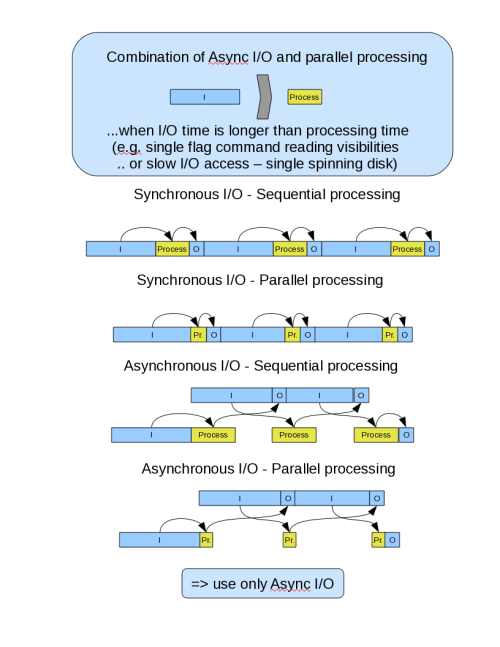
\includegraphics[scale=0.7]{async.parallel.diagram.IOdominates.png}
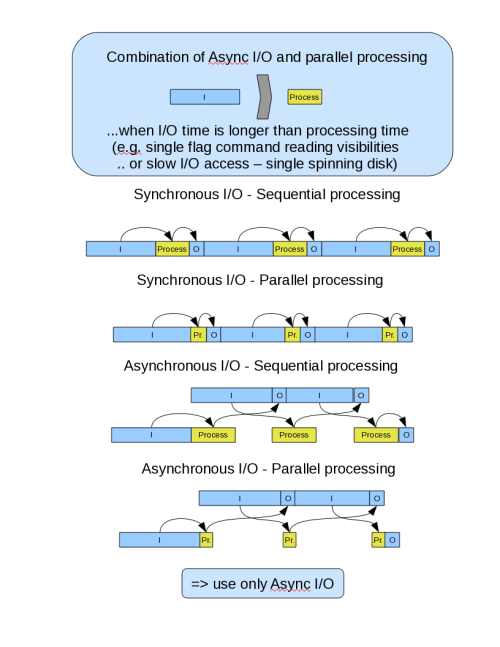
\includegraphics[scale=0.7]{async.parallel.diagram.IOdominates.png}
\caption{Explanation...}
\label{Fig:AsyncDiags}
\end{figure}






\subsubsection{Timing Tests}

Data : 

Continuum : few fat channels.\\
SpectralLine : many thin channels.\\

SinglePointing : contiguous scans on the same field\\
Mosaic  :  each scan is a different fields.\\

\begin{enumerate}
\item \label{dA} L-band continuum , Single Pointing   ----- need to decide dataset (probably G55.7+3.4\_1s.ms)
\item \label{dB} L-band spectral-line , Mosaic            ----- need to pick dataset 

\end{enumerate}


\paragraph{Comparison between modes}
%{\green Tables from Justo for 50 and 150 GB continuum datasets. }


\begin{figure}
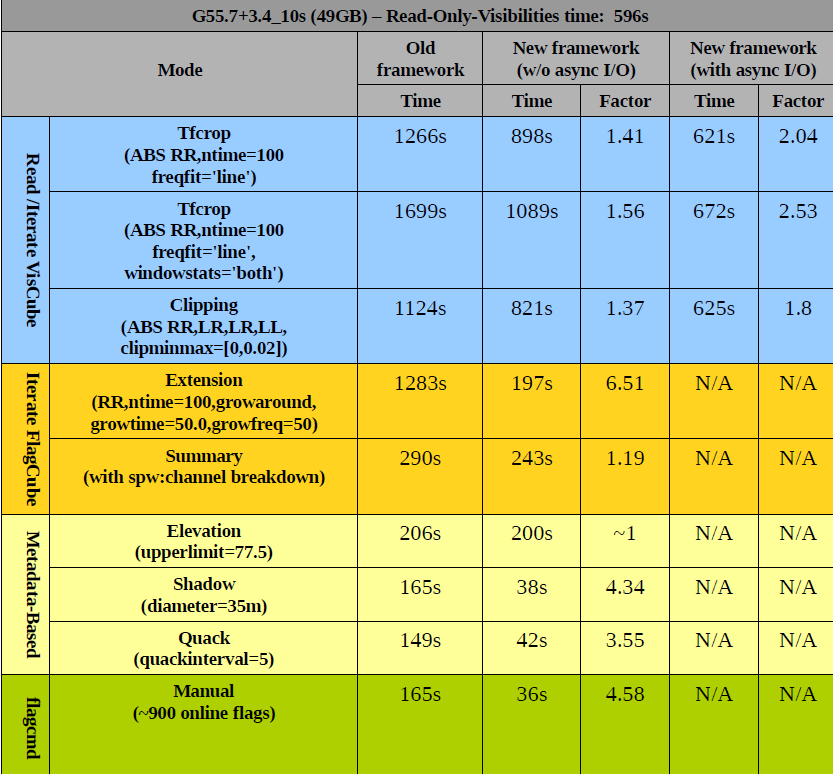
\includegraphics[scale=0.7]{table.timings.50GB.G55data.png}
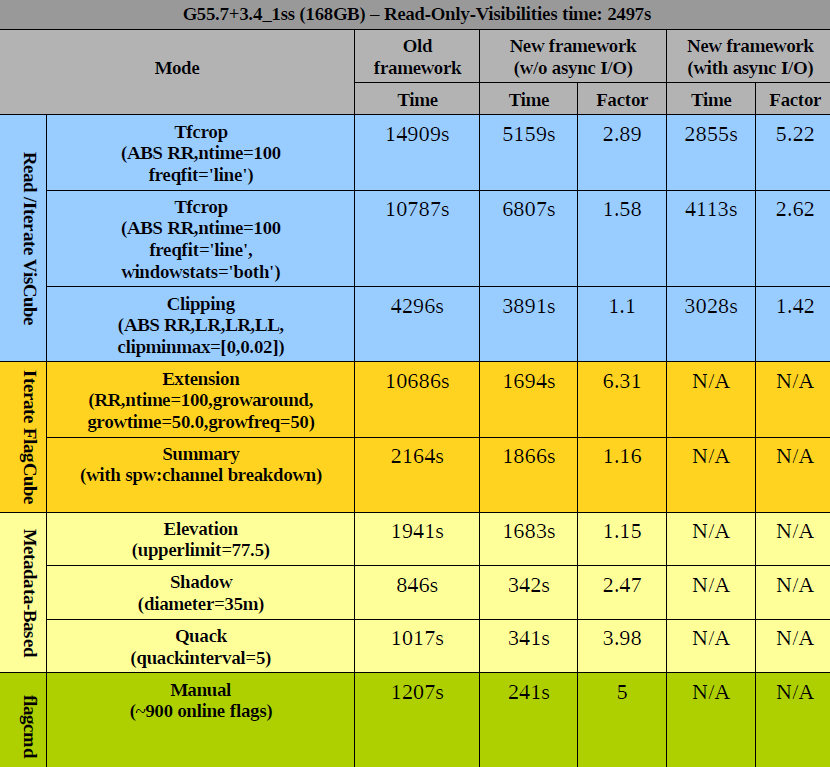
\includegraphics[scale=0.7]{table.timings.150GB.G55data.png}
\caption{These tables show timing comparisons between various modes, for two EVLA continuum datasets. Parameters of the datasets are... }
\end{figure}


\paragraph{Break-down of timings} : if possible, with and without async-IO.
\begin{enumerate}
\item  Only-reading-visibilities 
\item  Only-reading flags
\item  Only-writing flags
\item  (pls ignore if this makes no sense.) Only-iterating through the visbuffers without reading/writing anything (i.e. to see if much time is saved by the loose union). 
\end{enumerate}

\paragraph{Comparison between data-shapes and iteration patterns}

Two types of datasets : wideband continuum single-pointing,   spectral-line mosaic



%%%%%%%%%%%%%%%%%%%%%%%%%%%%%%%%%%%%%%%%%%%%%%%%%%%%
%%%%%%%%%%%%%%         SECTION           %%%%%%%%%%%%%%%%%%%%%%%%%%%
%%%%%%%%%%%%%%%%%%%%%%%%%%%%%%%%%%%%%%%%%%%%%%%%%%%%



\subsection{Python tool and task}\label{Sec:TaskTool}

\subsubsection{agentflagger tool}
\paragraph{Examples how to use the the new flagging framework from the tool.}
All the functions available in the tool are explained
\htmladdnormallink{here.}{http://www.eso.org/~scastro/ALMA/casa/active/CasaRef/agentflagger-Module.html}

\begin{enumerate}
\item Open the MS or a calibration file and attach it to the tool.

The function
takes three arguments, the MS or CAL table, the iteration approach to use and the time interval. 
Only the MS is mandatory to use. By default it will use the
FlagDataHandler::SUB\_INTEGRATION iteration approach and 0.0 seconds as the
time interval.

\begin{verbatim}
    af.open('my.ms')
\end{verbatim}

\item Select the data where to flag. If left blank, the whole MS will be
selected.

This step will use the MS Selection class. There are two functions to perform the
selection. One takes a Python dictionary (Record in C++) of the parameters, the
other takes the individual parameters as arguments.

\begin{verbatim}
  1) First method:
    selection={}
    selection['spw']="0:1~10"
    selection=['scan']="1"
    af.selectdata(selection)

  2) Second method:
    af.selectdata(spw="0:1~10", scan="1")
\end{verbatim}

\item Parse the parameters of the flagging agents.

Now it is time to build a list of the agents that we want to run to process the data. This
step will create a list of all the agents that will be executed to flag/unflag the data.
This method can be called multiple times. Every call should contain the desired parameters of
the agent and optionally data selection parameters. When data selection parameters are present,
the agent will only loop through that portion of the data.

This method will check if the requested agent (mode) is known from the following list
(manual, clip, quack, shadow, elevation, tfcrop, rflag, extend, unflag and summary). If
empty or unknown, it will give a warning and return.

If any tfcrop, rflag or extend mode is present, this method will calculate the maximum value
of time interval (ntime) from these agents. The maximum value will be used for
all the agents in the list.

A similar situation will happen with the combinescans parameter. If any of the combinescans is
True, it will be taken as True to all agents.

Async I/O will be activated if any of the modes clip, tfcrop or rflag is requested.

Only for the tfcrop agent, if a correlation ALL is requested, this method will create one
agent for each available polarization in the MS. For example, if the MS contains polarizations
XX and YY and the parameter is correlation="ABS\_ALL", then there will be two
tfcrop agents, one with correlation="ABS\_XX" and the other with
correlation="ABS\_YY". The apply parameter is set by default to True to apply
the flags.

\begin{verbatim}
     agent_pars = {}
     agent_pars["mode"] = "clip"
     agent_pars["clipzeros"] = true
     agent_pars["apply"] = true
     af.parseagentparameters(agent_pars)

     agent_pars = {}
     agent_pars["mode"] = "manual"
     agent_pars["autocorr"] = true
     af.parseagentparameters(agent_pars)

     agent_pars = {}
     agent_pars["mode"] = "summary"
     agent_pars["basecnt"] = true
     af.parseagentparameters(agent_pars)
\end{verbatim}

There are convenience functions to parse the agent's parameters, one specific for each agent.
The above calls can be done instead using these functions.

\begin{verbatim}
     af.parseclipparameters(clipzeros=true, apply=true)
     af.parsemanualparameters(autocorr=true)
     af.parsesummaryparameters(basecnt=true)
\end{verbatim}

In either one of the cases, three agents will be created. We need to initialize the agents, which
will call the constructor of each one of them and set the parameters that were given in the previous
calls. Some basic checks will be performed at this stage for types and values of the parameters.

If any tfcrop, rflag, extend or display agent is in the list, the iteration approach will be
set to a different value depending on whether combinescans is true or not. When True, the
iteration approach will be set to
FlagDataHandler::COMBINE\_SCANS\_MAP\_ANTENNA\_PAIRS\_ONLY, otherwise to
FlagDataHandler::COMPLETE\_SCAN\_MAP\_ANTENNA\_PAIRS\_ONLY.

\item Initialize the agents.

This method will create agents and add them to a FlagAgentList. If for any reason, the call to
FlagAgentBase::create(fdh\_p, agent\_rec) fails, an error message will be
displayed. Any agents previously added to the FlagAgentList will remain there. A subsequent call to this method can be done to add
more agents to the same FlagAgentList.

\begin{verbatim}
     af.init()
\end{verbatim}

\item Process the flags and write them to the MS.

The run method takes two parameters, writeflags and sequential.
The parameter writeflags controls whether to write the flags or not to the MS.
By default it is set to True. Setting writeflags to False is useful when one
wants to run the tool together with the display agent to see what is going to be
flagged before deciding to write or not to the MS. The sequential parameter
controls if the order of the agent's list is to be preserved or not. If set to
False, the order will not be preserved and the framework may execute the agent's list in parallel.
By default sequential is set to True.

The run method gathers several reports, depending on wich agents are run. The display and summary agents
produce reports that can be retrieved from calling the run method. The reports are returned via a Python
dictionary. When executed from the task, only the report of the
last summary in the list will be returned. If executed from the tool level,
multiple reports are allowed for the summary agent.

In the previous example, only one summary agent was added to the list, therefore
two reports will be returned in the dictionary. The first report contains the
summaries per field, spw, scan, correlation, etc. The second report
gives the antenna positions for plotting.

\begin{verbatim}
     my_reports = af.run()
\end{verbatim}

\item Destroy the tool.

\begin{verbatim}
    af.done()
\end{verbatim}
 \end{enumerate}
 
\paragraph{The following are only possible in the tool.}
\begin{enumerate}

\item Run multiple summary agents in a list. In order to do this, add as many
summary agents are desired when parsing the agent's parameters. You can do this by
calling the af.parseagentparameters() several times before calling af.init().

\item Determine to run the agents in sequential or in parallel. Set the
'sequential' parameter of the run method to True or False to control this.

\item Flag CAL tables in currently only possible in the tool. Give a CAL table
name when calling the af.open() method instead of a MS.

\end{enumerate}

\paragraph{Explain the heuristics applied for the automatic activation of async
I/O and parallel run}

\subsubsection{flaghelper functions}

This Python file contains many helper functions for flagdata and flacmd. The
functions can be imported inside casapy.

\begin{verbatim}
     import flaghelper as fh
\end{verbatim}

\subsubsection{flagdata task}
Help for the flagdata task is available \htmladdnormallink{here.}
{http://casa.nrao.edu/docs/taskref/flagdata-task.html}

\subsubsection{flagcmd task}
Help for the flagcmd task is available \htmladdnormallink{here.}
{http://casa.nrao.edu/docs/taskref/flagcmd-task.html}



%%%%%%%%%%%%%%%%%%%%%%%%%%%%%%%%%%%%%%%%%%%%%%%%%%%%





\section{The MSTransform framework}\label{Sec:Running}
% Add parts from Justo's document.
% I/O improvement by avoiding read/write to disk multiple times.
% order of running the transformations
% independence of each transformation.
% new VI???
Documentation for the task and tool can be found in:
\htmladdnormallink{Task Documentation}{http://casa.nrao.edu/docs/TaskRef/TaskRef.html}
\htmladdnormallink{Tool Documentation} {http://casa.nrao.edu/docs/CasaRef/CasaRef.html}

\subsection{Splitting capabilities}
Task mstransform behaves like split in all cases that concern sub-table re-indexing
and selection. It does not support multiple channel selections, which are separated by
a semi-colon. If there is an spw selection, it will re-index the spws starting from 0.

\subsection{Partition and Multi-MS support}
Task mstransform can do everything that task partition does and more. It supports
channel selections and re-indexing of spw sub-tables. The sub-tables are consolidated
in the output MMS, which does not happen in task partition. %Explain POINTING,SYSCAL tables

The user has the option to create an output MMS in parallel (using simple_cluster) or
in sequential. Set the parameter {\it parallel} to True to use simple_cluster. Note that
for small MSs, we recommend to create MMSs in sequential, as the overhead of creating
a cluster and managing the engines can become significant.

The combination of some transformations and createmms=True is not possible in
some cases, depending on the choice of {\it separationaxis}. The following table summarizes this:

\begin{verbatim}

separationaxis  combinespws  nspw > 1  regridms  chanaverage  timespan='scan' hanning
--------------------------------------------------------------------------------------
spw                NO         NO         YES        YES           YES           YES
scan               YES        YES        YES        YES           YES*          YES
both               NO         NO         YES        YES           YES*          YES

* --> we can partition per scan or scan,spw but cannot let timebins span changes in scan
      when timeaverage=True. The task will reset timespan to None in these cases.

\end{verbatim}

% Add the forbidden combinations of axis and transformations

\subsection{Combination of spectral windows}
Task mstransform can combine spectral windows independently or
with a reference frame transformation. When {\it combinespws} is set to True, the task will
combine all the selected spectral windows into one. The index of the output spw
will be 0. When there are overlapping channels, they will be averaged to form one
output channel.

\subsection{Channel averaging}
Similar to task split, mstransform can average the selected channels based on a
width parameter. The parameter {\it chanbin} can be either an integer or a list of
integers that will apply to each spw in the selection.

A parameter called {\it useweights} controls the type of weights to use in the
averaging. The options are flags that will consider the FLAG column and spectral
that will consider the WEIGHT_SPECTRUM column.

% use weights parameter

\subsection{Reference frame transformation}
The parameter {\it regridms} in mstransform can do many things. One can change the
reference frame based on the available sub-parameters and hence separate the spectral
windows into a regular grid of a given number of spws. This is a new feature in CASA
4.1 and can be applied in many use-cases. %(Expand and list some use-cases)

If {\it nspw} is greater than 1, the input spws will be separated into the given
number. If nchan is set, it will refer to the number of channels to have in each
separated spw. Note that internally, the framework will first combine the input
spws to take gaps and overlap into account, before separating them in the desired
number.

The regridms transformation differs from task cvel in a few cases. Task cvel has a
parameter {\it passall} to copy or not the non-selected spws into the output MS. In 
mstransform we only consider the {\it passall=False}, meaning that we only consider the
selected spws of the MS. Task cvel always combines spw when changing the reference
frame, while mstransform can do both cases. The combination of spectral windows in mstransform
is controlled by the independent parameter {\it combinespws}.

\subsection{Hanning smoothing}
Set the parameter {\it hanning} to True to Hanning smooth the MS. Contrary to the
hanningsmooth task, mstransform creates a new output MS and writes the smoothed transformation
to the DATA column of the output MS, not to the CORRECTED_DATA column.

Another difference with respect to the hanningsmooth task is that the transformation will be 
applied to all the data columns requested by the user in the parameter {\it datacolumn}. If the 
requested column does not exist, it will exit with an error. 

\subsection{Time averaging - To be implemented}
% Add stuff in here
%Similar to split, this task can average the MS in time, based on a set of parameters.

%timespan
%minbaselines
%quantize_c


\section{Examples}\label{Sec:Examples}
How to run the mstransform task for several common use-cases.

\begin{enumerate}
\item Split three spectral windows of a field from an MS.
\begin{verbatim}
mstransform(vis='inp.ms', outputvis='out.ms', datacolumn='data', spw='1~3', field='JUPITER')
\end{verbatim}
\item Combine four spectral windows into one.
\begin{verbatim}
mstransform(vis='inp.ms', outputvis='out.ms', combinespws=True, spw='0~3')
\end{verbatim}
\item Apply Hanning smoothing in MS with 24 spws. Do not combine spws.
\begin{verbatim}
mstransform(vis='inp.ms', outputvis='out.ms', hanning=True, datacolumn='data')
\end{verbatim}
\item Create a multi-MS in paralell with spw separation and channel selection.
\begin{verbatim}
mstransform(vis='inp.ms', outputvis='out.mms', spw='0~4,5:1~10', createmms=True,
            separationaxis='spw', parallel=True)
\end{verbatim}
\item Average channels in CORRECTED column using a bin of 3 channels in XX.
\begin{verbatim}
mstransform(vis='inp.ms', outputvis='out.ms', spw='0:5~16', correlation='XX', 
            freqaverage=True, freqbin=3)
\end{verbatim}
\item Combine spws and regrid MS to new channel structure. Average width is 2 channels.
\begin{verbatim}
mstransform(vis='inp.ms', outputvis='out.ms', datacolumn='DATA', field='11',
            combinespws=True, regridms=True, nchan=1, width=2)
\end{verbatim}
\item Regrid MS to new channel structure, change reference frame to BARY and set
new phasecenter to that of field 1. Use mode frequency for the parameters.
\begin{verbatim}
mstransform(vis='inp.ms', outputvis='out.ms', datacolumn='DATA', spw='0', field='1', 
            regridms=True, nchan=2, mode='frequency', width='3MHz', start='115GHz', 
            outframe='BARY', phasecenter=1)
\end{verbatim}
\item Set a custom tile shape for the output MS using the parameter tileshape. This will
set the tileshape to 4 correlations, 64 channels and 1024 rows.
\begin{verbatim}
mstransform(vis='inp.ms', outputvis='out.ms', tileshape=[4,64,1024])
\end{verbatim}
\item Separate a large input spw into a regular grid of 5 output spws, each with 10 channels.
\begin{verbatim}
mstransform(vis='inp.ms', outputvis='out.ms', spw='0', regridms=True, nchan=10, nspw=5)
\end{verbatim}



\end{enumerate}

\section{Frequently Asked Questions}\label{Sec:FAQ}
\begin{description}
  \item[Q1: How to run mstransform to mimic cvel?] \hfill 
  Set the parameter {\it regridms}I to True. If there is more than one spw in the
selection, set also {\it combinespws} to True because cvel always combines the selected
spws.

  \item[Q2: How to run mstransform to mimic split and the width parameter?] \hfill 
  To do channel average, set {\it chanaverage} to True and set {\it chanbin} to the
  appropriate value.

\end{description}




\end{document}


